\section{Introduction}
Computer aided evolution is becoming increasingly popular for tasks which involve creating models which have been optimized for certain characteristica.
Ultimately the goal with such evolution is to develop solutions which are not the most obvious design choices from a human perspective, but perform superior to already known solutions.\\

An example of such results are space antennas developed by Hornsby\cite{paper:ev4} using generative Computer-Automated Evolutionary Design[See figure \ref{fig:nasa_antenna}], which have rather controversal designs. While most antennas are somewhat straight in a direction these particular antennas are revolving around themselves in arbitrary directions.

\begin{figure}[ht]
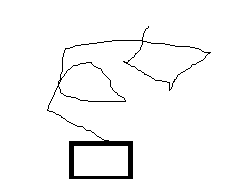
\includegraphics[scale=.7]{content/img/space_antenna}
\label{fig:nasa_antenna}\\
\caption{Image of the NASA Antenna \cite{paper:ev4} }
\end{figure}

Building from such previous experiences, that something which usually has a pretty standardized morphology in regards to design can get so fundamentally different results when applying EAs, leads us to wanting to apply such methodology to other domains.

The chosen domain is within furniture, namely the types which should be suited for seating.
%This project focusses on using computer aided evolution to generate models for furniture, particularly for the activity of sitting.

By tweaking the parameters to optimize for material or comfort, the candidate solutions might provide some very interesting and hopefully 'revolutionizing' designs.
